% PDF/A filecontents
\RequirePackage{filecontents}
\begin{filecontents*}{\jobname.xmpdata}
  \Title{Document’s title}
  \Author{Author’s name}
  \Language{it-IT}
  \Subject{The abstract, or short description.}
  \Keywords{keyword1\sep keyword2\sep keyword3}
\end{filecontents*}

\documentclass[12pt,                    % corpo del font principale
               a4paper,                 % carta A4
               twoside,                 % impagina per fronte-retro
               openright,               % inizio capitoli a destra
               english,                 
               italian,                 
               ]{book}    

%**************************************************************
% Importazione package
%************************************************************** 

\PassOptionsToPackage{dvipsnames}{xcolor} % colori PDF/A
\usepackage{colorprofiles}
\usepackage[a-2b,mathxmp]{pdfx}[2023/02/24]    % configurazione PDF/A.    validare in https://www.pdf-online.com/osa/validate.aspx
%\usepackage{amsmath,amssymb,amsthm}    % matematica
\usepackage[T1]{fontenc}                % codifica dei font: % NOTA BENE! richiede una distribuzione *completa* di LaTeX
\usepackage[utf8]{inputenc}             % codifica di input; anche [latin1] va bene % NOTA BENE! va accordata con le preferenze dell'editor
\usepackage[english, italian]{babel}    % per scrivere in italiano e in inglese; % l'ultima lingua (l'italiano) risulta predefinita
\usepackage{bookmark}                   % segnalibri
\usepackage{caption}                    % didascalie
\usepackage{chngpage,calc}              % centra il frontespizio
\usepackage{csquotes}                   % gestisce automaticamente i caratteri (")  %guida tesi dice di opzioni [autostyle,italian=guillemets] che servono con biblatex 
\usepackage{emptypage}                  % pagine vuote senza testatina e piede di pagina
\usepackage{epigraph}			              % per epigrafi
\usepackage{eurosym}                    % simbolo dell'euro
%\usepackage{indentfirst}               % rientra il primo paragrafo di ogni sezione %sotto c'è il comando \parindent impostato a 0 pt
\usepackage{graphicx}                   % immagini
\usepackage{hyperref}                   % collegamenti ipertestuali
\usepackage[binding=7mm]{layaureo}      % margini ottimizzati per l'A4; rilegatura di 5 mm  %IRE: modificata io a 7
\usepackage{listings}                   % codici
\usepackage{microtype}                  % microtipografia
\usepackage{mparhack,fixltx2e,relsize}  % finezze tipografiche
\usepackage{nameref}                    % visualizza nome dei riferimenti                                      
\usepackage[font=small]{quoting}        % citazioni
\usepackage{subfig}                     % sottofigure, sottotabelle
\usepackage[italian]{varioref}          % riferimenti completi della pagina
\usepackage{booktabs}                   % tabelle                                       
\usepackage{tabularx}                   % tabelle di larghezza prefissata                                    
\usepackage{longtable}                  % tabelle su più pagine                                        
\usepackage{ltxtable}                   % tabelle su più pagine e adattabili in larghezza
\usepackage{setspace}                   % IRE spaziatura tra le linee, sotto è scritto il comando singlespacing, onehalfspacing, douplepspacing, libera teoricamente va racchiuso tra begin e end (spacing)(x)
\usepackage{fancyhdr}                   % IRE Extensive control of page headers and footers
\usepackage{float}                      % IRE permette di modificare il modo con cui gli ambienti tradizionali vengono composti, introducendo il concetto di stile per questi oggetti ‘galleggianti’ come immagini e tabelle.
%\usepackage{charter}                   % IRE
\usepackage{subfig}                     % IRE !!prerequisito pacchetto caption!!  permette di affiancare più figure o tabelle dando a ciascuna una sottodidascalia
%\usepackage[toc, acronym]{glossaries}   % glossario
%\usepackage[backend=biber,style=verbose-ibid,hyperref,backref]{biblatex} %bibliografia
\usepackage{tablefootnote}              % IRE pacchetto per le note in tabella

\hypersetup{
    %hyperfootnotes=false,
    %pdfpagelabels,
    %draft,	% = elimina tutti i link (utile per stampe in bianco e nero)
    colorlinks=false, %IRE cambiato
    linktocpage=true,
    pdfstartpage=1,
    pdfstartview=,
    % decommenta la riga seguente per avere link in nero (per esempio per la stampa in bianco e nero)
    %colorlinks=false, linktocpage=false, pdfborder={0 0 0}, pdfstartpage=1, pdfstartview=FitV,
    breaklinks=true,
    pdfpagemode=UseNone,
    pageanchor=true,
    pdfpagemode=UseOutlines,
    plainpages=false,
    bookmarksnumbered,
    bookmarksopen=true,
    bookmarksopenlevel=1,
    hypertexnames=true,
    pdfhighlight=/O,
    %nesting=true,
    %frenchlinks,
    %urlcolor=webbrown, IRE
    %linkcolor=RoyalBlue, IRE
    %citecolor=webgreen, IRE
    %pagecolor=RoyalBlue,
    %urlcolor=Black, linkcolor=Black, citecolor=Black, %pagecolor=Black,
    pdftitle={\myTitle},
    pdfauthor={\textcopyright\ \myName, \myUni, \myFaculty},
    pdfsubject={},
    pdfkeywords={},
    pdfcreator={pdfLaTeX},
    pdfproducer={LaTeX}
}
%\definecolor{webgreen}{rgb}{0,.5,0} IRE
%\definecolor{webbrown}{rgb}{.6,0,0} IRE
\definecolor{footer-gray}{HTML}{808080}
\onehalfspacing %IRE imposto il pacchetto setspace spaziatura tra le linee: singlespacing, onehalfspacing, douplepspacing
\parindent=0pt %IRE Rientro della prima riga.
\pagestyle{fancy}
\fancyhf{}
\rhead{\textcolor{footer-gray}{Tesi}}
%\lhead{\textcolor{footer-gray}{Sweven Team}}
\fancyfoot{}
\rfoot{\textcolor{footer-gray}{\thepage}}
%\renewcommand*\contentsname{Indice} %%IRE mi sembra inutile, era in Sweven sopra indice e paragrafi
\setcounter{tocdepth}{5}	%aggiunge paragrafi e sottoparagrafi all'indice
\setcounter{secnumdepth}{3}	%indica fino a che numero indicizazzare nell'indice con 0.0.xxx (5 indica fino a sottoparagrafi, 3 fino a subsubsection)
\newcommand{\glossario}[1]{\textit{#1}\textsubscript{\textit{G}}}  %glossario con l'indice basso G                                 
\newcommand{\myTitle}{Creazione di applicazioni low-code in ambiente Microsoft}
\newcommand{\myDegree}{Tesi di laurea}
\newcommand{\myUni}{Università degli Studi di Padova}
\newcommand{\myFaculty}{Corso di Laurea in Informatica}
\newcommand{\myDepartment}{Dipartimento di Matematica "Tullio Levi-Civita"}
\newcommand{\profTitle}{Prof.ssa }
\newcommand{\myProf}{Ombretta Gaggi}
\newcommand{\myName}{Irene Benetazzo} %correggere nel frontespizio "laureanda" se femmina
\newcommand{\myCode}{1223865}
\newcommand{\myLocation}{Padova}
\newcommand{\myAA}{2022-2023}
\newcommand{\myTime}{Febbraio 2023}


\begin{document}
\begin{titlepage}

    \begin{center}
    
    \begin{LARGE}
    \textbf{\myUni}\\
    \end{LARGE}
    
    \vspace{10pt}
    
    \begin{Large}
    \textsc{\myDepartment}\\
    \end{Large}
    
    \vspace{10pt}
    
    \begin{large}
    \textsc{\myFaculty}\\
    \end{large}
    
    \vspace{20pt}
    \begin{figure}[htbp]
    \begin{center}
    
\includegraphics[height=6cm]{immagini/logo-unipd.png}
    \end{center}
    \end{figure}
    \vspace{-10pt} 
    
    \begin{LARGE}
    \begin{center}
    \textbf{Creazione di applicazioni low-code \\ in ambiente Microsoft}\\
    \end{center}
    \end{LARGE}
    
    \vspace{10pt} 
    
    \begin{large}
    \textsl{\myDegree}\\
    \end{large}
    
    \vspace{20pt} 
    
    \begin{large}
    \begin{flushleft}
    \textit{Relatore}\\ 
    \vspace{5pt} 
    \profTitle \myProf
    \end{flushleft}
    
    \vspace{0pt} 
    
    \begin{flushright}
    \textit{Laureanda}\\
    \vspace{5pt} 
    \myName\\
    \myCode
    \end{flushright}
    \end{large}
    
    \vspace{40pt}
    
    \line(1, 0){338} \\
    \begin{normalsize}
    \textsc{Anno Accademico \myAA}
    \end{normalsize}
    
    \end{center}
    \end{titlepage}

%DOPO IL FRONTESPIZIO
\clearpage
\phantomsection
\thispagestyle{empty}
\hfill
\vfill
\noindent\myName: \textit{\myTitle,}\\
\myDegree,
\textcopyright\ \myTime.
\newpage

%Citazione e ringraziamenti\\
%Organizzazione del testo\\
%Indice, tabelle, figure\\
%Introduzione\\
%Capitolo 1\\
%\dots\\
%Conclusioni\\
%Inseriamo una nota\footnote{nota di prova, vediamo se descrizione lunga tutta la riga cosa succede con la linea sopra} \\
%\textsc{Eventuali appendici}\\
%\glossario{Glossario}\\
%Bibliografia\\
%Fine\\

\frontmatter
\begingroup
    %\chapter{Sommario}
    %\clearpage
    %\let\cleardoublepage\relax
    %\chapter{Ringraziamenti}
    %\clearpage
    \tableofcontents
    \clearpage
    \let\cleardoublepage\relax
    \listoffigures
    \clearpage
    \listoftables
    \clearpage
\endgroup

\mainmatter
\chapter{Introduzione}
\section{Presentazione azienda}
L'azienda Alfa\footnote{Alfa nome di fantasia  per richiesta esplicita dell'azienda} viene fondata nel 1964 in un paese nella provincia di Padova specializzandosi in prodotti per l'essiccamento e la filtrazione.
Successivamente apre altre sedi anche all'estero in Europa, negli anni novanta prima viene comprata da un'azienda inglese e dopo pochi anni da un'azienda americana.
Attualmente è una multinazionale con sede in America e sedi operative in 48 paesi di tutti i continenti. 
In provincia di Padova si è sempre lavorato principalmente prodotti per essiccamento e filtrazione che rappresentano un ramo dell’azienda, ma l’azienda produce in tantissimi ambiti: aerospaziale, elettromeccanica, climatizzazione, idraulica, pneumatica, gestione di fluidi e gas, controllo di processo, sigillatura e schermatura.
\section{Obiettivo stage}
L'obiettivo di questo stage è sviluppare due applicazioni mobile su piattaforma Microsoft che offre la possibilità di creare soluzioni low-code.
Lo scopo delle applicazioni è dare la possibilità ai dipendenti di velocizzare alcune operazioni come la visualizzazione dei dati e la registrazione delle attività svolte in giornata.

\section{Organizzazione e convenzioni del testo}
La tesi descrive tre applicazioni e di conseguenza i capitoli sono spesso suddivisi in quattro sezioni:
la prima parte comune, la seconda dedicata all'applicazione per i dati del magazzino, la terza dedicata all'applicazione per il personale dell'information technology (IT) e la quarta dedicata all'applicazione per l'inserimento richieste ordini.\\
La tesi prevede sette capitoli, di cui il primo è questo cioè l'introduzione in cui si presenta l'azienda, lo stage e i prodotti che verranno sviluppati. \\
Il \textbf{secondo capitolo} illustra le tecnologie che verranno utilizzate durante lo stage.\\
Il \textbf{terzo capitolo} identifica i requisiti delle applicazioni classificandoli in funzionali, qualitativi e di vincolo; insieme al proponente e committente si è stabilito se sono obbligatori, desiderabili o facoltativi.\\
Il \textbf{quarto capitolo} descrive la fase di progettazione delle applicazioni.\\
Il \textbf{quinto capitolo} descrive la fase di sviluppo delle applicazioni, riportando in dettaglio le parti più significative.\\
Il \textbf{sesto capitolo} descrive la fase di test ed illustra gli obiettivi raggiunti.\\
Il \textbf{settimo capitolo} contiene le considerazioni finali sul progetto di stage.\\
Nella stesura del documento sono state utilizzate le seguenti convenzioni tipografiche:
\begin{itemize}
    \item Il pedice G indica che la spiegazione di quel \glossario{termine}, scritto in corsivo, è presente nel glossario.
    \item Il numero inserito come apice indica che è presente la relativa nota a fine pagina.
    \item Il codice e le formule riportate verranno scritte mediante il seguente \texttt{font dattilografico} seguite dalla descrizione in \textit{corsivo}.    
\end{itemize}

\section{Applicazione per i dati del magazzino}
\subsection{Situazione iniziale}
Gli operatori di magazzino con la semplice necessità di visualizzare alcuni dati, come la locazione di un determinato articolo, devono necessariamente usare un computer per accedere al sistema aziendale \glossario{ERP} che è implementato senza un’interfaccia grafica. 
Inoltre l’operatore in magazzino non ha un suo computer personale ma è presente soltanto qualche postazione fissa di computer.
\subsubsection{Enterprise Resource Planning (ERP)}
ERP è un sistema che si occupa della gestione e pianificazione aziendale delle risorse integrando tutti i moduli aziendali: amministrazione, contabilità, produzione, magazzino, logistica, acquisti, vendite, etc…
L’avere tutto insieme con una sincronizzazione continua ben organizzata incrementa la produttività, ottimizza la gestione dei materiali e le fasi di produzione, agevolando anche il coordinamento.

\subsection{Obiettivo}
L'obiettivo è facilitare, modernizzare e velocizzare l’accesso alla visualizzazione dei dati creando un’applicazione installabile in qualsiasi dispositivo mobile (smartphone o tablet). 
In azienda è già molto utilizzato l’ambiente Microsoft, quindi si è pensato di utilizzare PowerPlatform, in particolare Power Apps.


\section{Applicazione per il personale IT}
\subsection{Situazione iniziale}
I dipendenti del personale information technology non utilizzavano nessuna applicazione, form o altro metodo per registrare le attività svolte durante la giornata di lavoro.
\subsection{Obiettivo}
L'obiettivo è fornire una semplice applicazione, usabile da qualsiasi dispositivo elettronico, per compilare il form e registrare le proprie attivià svolte o visualizzare i dati inseriti avendo la possibilità di modificarli o eliminarli; inoltre, i dirigenti, desiderano avere la visualizzazione grafica dei dati.


\section{Applicazione per l'inserimento richieste ordini}
\subsection{Situazione iniziale}
I dipendenti della sede aziendale inserivano la richiesta dell'ordine direttamente nella lista, avvisavano manualmente tramite mail l'approvatore e il segretario che la processava burocraticamente. Inoltre avendo libero accesso alla lista tutto era visibile e modificabile da tutti.
\subsection{Obiettivo}
L'obiettivo è creare un'applicazione per agevolare e modernizzare l'inserimento della richiesta, creare un ciclo per automatizzare le varie fasi per l'approvazione della richiesta di un'ordine.


\chapter{Tecnologie}
In questo capitolo si illustrano tutte le tecnologie, software, servizi utilizzati per sviluppare le applicazioni.\\
Si preferisce realizzare un capitolo unico, sia per una panoramica maggiore, sia per evitare le ripetizioni delle descrizioni tecnologiche per ogni applicazione.
Mentre nel specifico capitolo dell'applicazione è presente un elenco di ciò che si è utilizzato.
\section{PowerPlatform} \label{tec:PowerPlatform}
PowerPlatform è una piattaforma Microsoft che racchiude vari strumenti per agevolare l’organizzazione usando strumenti innovativi e basati sul principio low-code.
Offre tantissimi modelli di qualsiasi tipologia da cui partire per creare ciò che si desidera.
Inoltre si ha molta scelta per caricare i dati sia da altri strumenti Microsoft sia da servizi esterni o anche da origini locali. \newline
Power Platform offre i seguenti software, alcuni solo online altri anche in versione dsektop dove permettono maggiori personalizzazioni.\\
Per l'illustrazione dei loghi della piattaforma si veda la \figurename \space \ref*{fig:PowerPlatform}.
\begin{figure}[h]
    \centering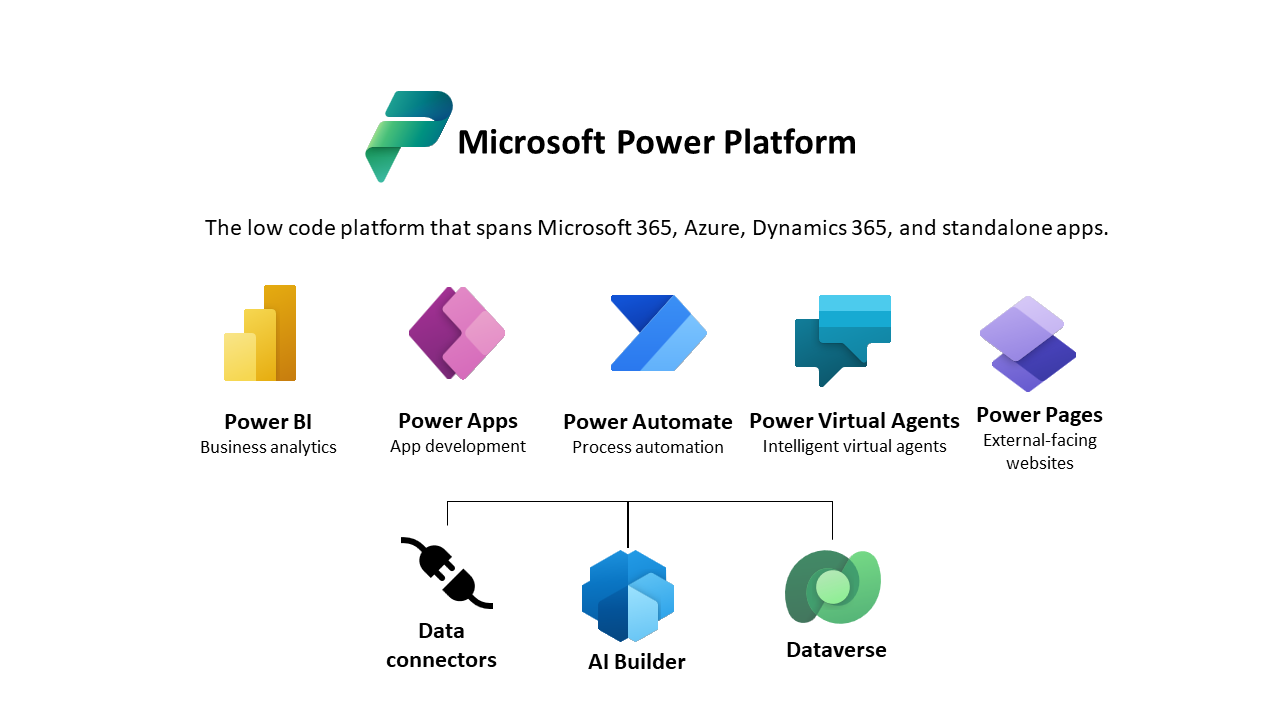
\includegraphics[width=\textwidth, height=\textheight,keepaspectratio]{immagini/Icone-PowerPlatform.png}
    \caption{Loghi PowerPlatform}
    \label{fig:PowerPlatform}
\end{figure}
\begin{description}
    \item \textbf{Power BI:} \label{tec:Power BI} permette l’analisi in autonomia di molti dati con parecchi strumenti per personalizzare la gestione e la visualizzazione anche mediante le funzionalità di intelligenza artificiale.
    \item \textbf{Power Apps:} \label{tec:Power Apps} permette di creare rapidamente applicazioni da zero o da modelli, il codice è necessario solo per impostare le proprietà degli elementi aggiunti.
    \item \textbf{Power Automate:} \label{tec:Power Automate} permette di automatizzare i processi organizzativi tramite l’impostazione di flussi che si attivano al seguito di un evento o in maniera ricorrente.
    \item \textbf{Power Virtual Agents:} permette di creare velocemente dei chatbot basati sull’intelligenza artificiale con anche la possibilità di usare più lingue.
    \item \textbf{Power Pages:} permette di creare rapidamente siti web, offre la possibilità di raccogliere i dati dei visitatori mediante Microsoft Dataverse.
\end{description}

\section{SharePoint} \label{tec:SharePoint}
SharePoint è una piattaforma di collaborazione, sviluppata da Microsoft, che permette di creare \glossario{intranet} tra membri dello stessa divisione, progetto agevolando la condivisione di materiale, la comunicazione, la creazione di applicazioni, siti personalizzati e liste condivise.
Inoltre permette molta personalizzazione anche per la tipologia di accesso ad ogni elemento per ogni membro; per il logo si veda la \figurename \space \ref*{fig:SharePoint}. 
In particolare SharePoint offre la possibilità di creare e condividere liste mediante il software Microsoft Lists.
\begin{figure}[H]
    \centering\includegraphics[width=0.2\textwidth, height=0.2\textheight,keepaspectratio]{immagini/logo-SharePoint.png}
    \caption{Logo SharePoint}
    \label{fig:SharePoint}
\end{figure}

\subsection{Microsoft Lists} \label{tec:Microsoft Lists}
è un servizio molto semplice e intuitivo con cui poter creare una lista di record in cui si può scegliere se visualizzare le colonne già previste di default o aggiungere nuove colonne specificando anche la tipologia di dato che verrà inserito. Per il logo si veda la \figurename \space \ref*{fig:M-Lists}.
\begin{figure}[H]
    \centering
\includegraphics[width=0.2\textwidth, height=0.2\textheight,keepaspectratio]{immagini/logo-MicrosoftLists2.png}
    \caption{Logo Microsoft Lists}
    \label{fig:M-Lists}
\end{figure}

\section{Microsoft SQL} \label{tec:Microsoft SQL}
Microsoft SQL Server, prodotto da Microsoft, è uno dei RDBMS\footnote{Relation Database Management System} più diffusi al mondo. 
Utilizza una variante del linguaggio SQL\footnote{Structured Query Language} standard, Transact-SQL sviluppato da Microsoft stesso; per il logo si veda la \figurename \space \ref*{fig:M-SQL}.
\begin{figure}[H]
    \centering
\includegraphics[width=0.3\textwidth, height=0.3\textheight,keepaspectratio]{immagini/logo-SqlServer.png}
    \caption{Logo Microsoft Sql Server}
    \label{fig:M-SQL}
\end{figure}

\section{DB2} \label{tec:DB2}
DB2 è un Relational Database Management System della IBM che permette di archiviare, gestire una grande mole di dati garantendo elevate prestazioni ed alta affidabilità con transazioni a bassa latenza.
Si utilizzano i comandi SQL\textsuperscript{1} per interrogare il database; per il logo si veda la \figurename \space \ref*{fig:DB2}.
\begin{figure}[H]
    \centering
\includegraphics[width=0.2\textwidth, height=0.2\textheight,keepaspectratio]{immagini/logo-ibm-db2.jpg}
    \caption{Logo DB2}
    \label{fig:DB2}
\end{figure}

\chapter{Analisi dei Requisiti}
Le richieste dei proponenti per le applicazioni sono state suddivise in requisiti funzionali, qualitativi o di vincolo; inoltre sono stati classificati in obbligatori, desiderabili o facoltativi.\\
La classificazione dei requisiti verrà identificata tramite il seguente codice che viene descritto nella \tablename \space \ref*{tab:Requisiti}.
\begin{center}
  \textbf{R[TIPO][PRIORITA'][NUMERO]-[APPLICAZIONE]}
\end{center}

\renewcommand{\arraystretch}{1.1} %aumento ampiezza righe
\begin{table}[H]
\begin{tabular}{ |m{8em}|m{26em}| }
  \hline
  \textbf{Nome} & \textbf{Descrizione} \\
  \hline
  R & Acronimo di Requisito \\
  \hline
  TIPO & Indica il tipo di requisito: \\
        & \textbf{F}: Requisto funzionale, definizione di una caratteristica necessaria nel software \\
        &	\textbf{V}: Requisito di vincolo, rappresenta un vincolo avanzato \\
        &	\textbf{Q}: Requisito di qualità, inerente le regole di qualità \\
  \hline
  PRIORITA' & Indica il tipo di priorità: \\
        &	\textbf{O}: Requisito obbligatorio \\
        &	\textbf{D}: Requisito desiderabile \\
        &	\textbf{F}: Requisito facoltativo \\
  \hline
  NUMERO & Codice Numerico Identificativo \\
  \hline
  APPLICAZIONE & Indica per quale : \\
               & \textbf{M}: Applicazione per i dati del magazzino \\
               & \textbf{IT}: Applicazione per il personale information technology \\
               & \textbf{OR}: Applicazione per l'inserimento richieste ordini \\
  \hline
\end{tabular}
\caption{Classificazione requisiti}
\label{tab:Requisiti}
\end{table}

\renewcommand{\arraystretch}{1.3} %aumento ampiezza righe
\section{Applicazione per i dati del magazzino}
L'applicazione per i dati del magazzino ha lo scopo di agevolare gli operatori nella visualizzazione delle informazioni di un articolo. Recuperati dal database sul server i dati vengono resi visualizzabili in un'applicazione per qualsiasi dispositivo. \\
Nella \tablename \space \ref*{tab:Requisiti-M} sono presentati i requisiti di questa applicazione.
\begin{table}[H]
  \begin{tabular}{ |m{6em}|m{28em}| }
    \hline
    \textbf{Codice} & \textbf{Descrizione requisito} \\
    \hline
    \textbf{RFO01-M} & Applicazione sviluppata per smartphone e tablet \\
    \hline
    \textbf{RFO02-M} & Sincronizzazione frequente con il sistema aziendale \glossario{ERP} \\
    \hline
    \textbf{RFO03-M} & La lettura del codice articolo tramite scannerizzazione \\
    \hline
    \textbf{RFO04-M} & Elenco delle informazioni obbligatorie da visualizzare:
          \begin{itemize}
          \begin{spacing}{1.0}
            \item descrizione dell'articolo;
            \item giacenza totale;
            \item quantità ordinata;
            \item quantità scaffale;
            \item operatore che acquista;
            \item fornitore;
            \item messaggio;
            \item tipo di locazione;
            \item locazione.
          \end{spacing}
          \end{itemize}\\
    \hline
    \textbf{RFD05-M} & Elenco delle informazioni desiderabili da visualizzare:
          \begin{itemize}
          \begin{spacing}{1.0}
            \item scorta minima;
            \item giacenza specifica per locazione.
          \end{spacing}
          \end{itemize} \\
    \hline
    \textbf{RVO01-M} & Applicazione sviluppata in ambiente Microsoft con \glossario{Power Apps} \\
    \hline
    \textbf{RQO01-M} & Ricevere la risposta dal database entro 5 secondi \\
    \hline
    \textbf{RQD02-M} & Applicazione sviluppata in un'unica schermata \\
    \hline
  \end{tabular}
\caption{Classificazione requisiti dell'applicazione dati del magazzino}
\label{tab:Requisiti-M}
\end{table}


\renewcommand{\arraystretch}{1.5} %aumento ampiezza righe
\section{Applicazione per il personale IT}
Lo scopo dell’applicazione è registrare le attività giornaliere effettuate dai dipendenti dell'information technology.\\
La visualizzazione grafica permette di valutare le migliori strategie, bilanciamento e organizzazione da adottare nel futuro prossimo. 
E' importante analizzare principalmente l’ultimo periodo e non tutto lo storico delle attività registrate.\\
I requisiti dell'applicazione sono presentati e classificati mediante la \tablename \space \ref*{tab:Requisiti-IT}. 
\begin{table}[H]
  \begin{tabular}{ |m{6em}|m{28em}| }
    \hline
    \textbf{Codice} & \textbf{Descrizione requisito} \\
    \hline
    \textbf{RFO01-IT} & Inserimento dell’attività specificando per quale organizzazione \\
    \hline
    \textbf{RFO02-IT} & Divieto di inserimento anticipato di attività future \\
    \hline
    \textbf{RFO03-IT} & Modifica ed eliminazione solo delle proprie attività \\
    \hline
    \textbf{RFO04-IT} & Eliminazione automatica degli inserimenti di oltre un anno prima \\
    \hline
    \textbf{RFD05-IT} & Filtri nella visualizzazione grafica dei dati \\
    \hline
    \textbf{RVO01-IT} & Applicazione sviluppata in ambiente Microsoft \\
    \hline
    \textbf{RVO02-IT} & La raccolta dei dati tramite \glossario{Microsoft Lists} \\
    \hline
    \textbf{RVO03-IT} & Visualizzazione grafica dei dati in \glossario{Power Bi} \\
    \hline
    \textbf{RQD01-IT} & Schermata home di benvenuto nell’applicazione \\
    \hline
    \textbf{RQF02-IT} & Filtri per agevolare la ricerca delle proprie attività inserite \\
    \hline
  \end{tabular}
\caption{Classificazione requisiti dell'applicazione dati del magazzino}
\label{tab:Requisiti-IT}
\end{table}
\newpage

\renewcommand{\arraystretch}{1.2} %aumento ampiezza righe
\section{Applicazione per l'inserimento richieste ordini}
I requisiti dell'applicazione sono presentati e classificati mediante la \tablename \space \ref*{tab:Requisiti-ON}
  \begin{table}[H]
    \begin{tabular}{ |m{6em}|m{28em}| }
      \hline
      \textbf{Codice} & \textbf{Descrizione requisito} \\
      \hline
      \textbf{RFO01-ON} & Applicazione sviluppata principalmente per pc \\
      \hline
      \textbf{RFO02-ON} & Visualizzabile lo stato della richiesta e numero ON\tablefootnote{Order Number, sigla interna dell'azienda.} \\
      \hline
      \textbf{RFO03-ON} & Elenco delle informazioni da inserire:
            \begin{itemize}
            \begin{spacing}{1.0}
              \item oggetto;
              \item progetto (menù a tendina);
              \item costo;
              \item attendibilità del costo;
              \item fornitore e codice (menù a tendina);
              \item data consegna prevista;
              \item codice conto (menù a tendina);
              \item quantità;
              \item note da includere nell'ordine;
              \item allegati.
            \end{spacing}
            \end{itemize}\\
      \hline
      \textbf{RFO04-ON} & Avvio automatico del ciclo di approvazione\\
      \hline
      \textbf{RFO05-ON} & Dopo l'approvazione in automatico mail al segretario\\
      \hline
      \textbf{RFO06-ON} & Il segretario inserisce il numero di riferimento dell'ordine (ON)\\
      \hline
      \textbf{RFO07-ON} & Solo approvatore e segretario possono modificare le richiesta\\
      \hline
      \textbf{RFD08-ON} & Nell'applicazione siano visualizzabili solo le proprie richieste\\
      \hline
      \textbf{RQO01-ON} & Inserimento della richiesta in modo agevole \\
      \hline
      \textbf{RQO02-ON} & Il richiedente viene costantemente aggiornato durante il ciclo\\
      \hline
      \textbf{RQD03-ON} & Nella mail inviata all'approvatore siano presenti direttamente i tasti per approvare o rifiutare una richiesta\\
      \hline
    \end{tabular}
  \caption{Classificazione requisiti dell'applicazione per l'inserimento richieste ordini}
  \label{tab:Requisiti-ON}
  \end{table}
  \renewcommand{\arraystretch}{1.5} %aumento ampiezza righe
\chapter{Progettazione}
\section{Applicazione per i dati del magazzino}
Il sistema aziendale \glossario{ERP} è basato su database \glossario{DB2} che si trovano sui server
aziendali in Inghilterra. Sono macchine IBM con il sistema operativo OS400, un sistema nato negli
anni ottanta in cui si dialoga sempre con uno strato software e mai direttamente con l’hardware
della macchina, ciò lo rende inattaccabile dai virus e hacker. Questo sistema si usa principalmente
per la gestione dei database, è molto veloce al suo interno ma un suo svantaggio è la lentezza
nell’estrarre i dati dall’esterno. Per connettersi dall’esterno si può usare un connettore di tipo \glossario{ODBC}
da cui si può creare una vista logica virtuale oppure si esportano i dati che vengono
salvati nei server locali; tra questi due server deve essere schedulato un aggiornamento frequente.\\
Infine Power Apps si connette direttamente al cloud di SQL Server, l’applicazione con un’unica
schermata visualizza solo le informazioni relative al codice articolo scansionato. Tutti i vari passaggi
richiedono l’accesso ai singoli database criptati mediante specifico utente e password per garantire
maggiore sicurezza.\\
Si è deciso di usare un’applicazione sviluppata mediante Power Apps di
Microsoft in quanto in azienda è il sistema principale e tutti i dipendenti, operai possiedono il
proprio account Microsoft personale con licenza completa.

\newpage

\section{Applicazione per il personale IT}
I dipendenti degli uffici information technology inseriscono le proprie attività svolte tramite il form presente nell’applicazione in \glossario{PowerApps}, ogni utente visualizza solo le proprie attività con possibilità di modificarle o eliminarle. 
Ogni attività registrata viene salvata in una lista di \glossario{Microsoft Lists}.\\
Lo scopo principale è di monitorare la produttività dell’ultimo periodo quindi si è stabilito di prevedere l’eliminazione automatica delle attività dopo un anno tramite un flusso Power Automate.
Per facilitare l’analisi della produttività e una visione a colpo d’occhio si è progettata una dashboard grafica interattiva che selezionando le singole voci permette di vedere, direttamente nel grafico, le relative distribuzioni per tipologia.

\section{Applicazione per l'inserimento richieste ordini}
I dipendenti della sede aziendale tramite il \glossario{form} nell’applicazione in \glossario{PowerApps} inseriscono la richiesta di un ordine specificando tutte le relative informazioni. 
All’inserimento della richiesta, oltre a salvarsi su una lista Microsoft, tramite \glossario{PowerAutomate} si avvia il ciclo di approvazione inviando una mail all’approvatore. 
Se approvato, oltre alla comunicazione al richiedente, automaticamente si genera la mail per il segretario burocratico che completerà la richiesta inserendo il numero d'ordine relativo e viene comunicato via mail al richiedente. 
Mentre se la richiesta viene rifiutata viene comunicato al richiedente e il ciclo termina.
\chapter{Sviluppo}
\section{Applicazione per i dati del magazzino}
Nei server aziendali in Inghilterra, al fine di agevolare la successiva estrazione dei dati e visto che effettuare le operazioni direttamente dentro il sistema \glossario{OS400} è molto più rapido, si crea una nuova tabella nel database \glossario{DB2} in cui viene effettuato il \glossario{join} tra le varie origini dei dati effettuando anche le somme di alcuni campi al fine di avere numeri con informazioni più dirette e semplici, infine si selezionano solo le colonne utili.
Il file ottenuto contiene più di cento mila record ed è già il risultato finale desiderato in cui si vorrebbe effettuare la ricerca del codice articolo per le relative informazioni.\\ 
Mediante il \glossario{connettore ODBC} si è creata una connessione \glossario{Linked Server} e tramite il codice scritto in \glossario{Microsoft SQL} si importa la tabella sul server di Padova.\\
Tra i due server è stato schedulato un aggiornamento ogni 15 minuti durante l’orario lavorativo, si veda la \figurename \space \ref*{fig:M-Schedulazione} per la schedulazione.
\begin{figure}[H]
    \centering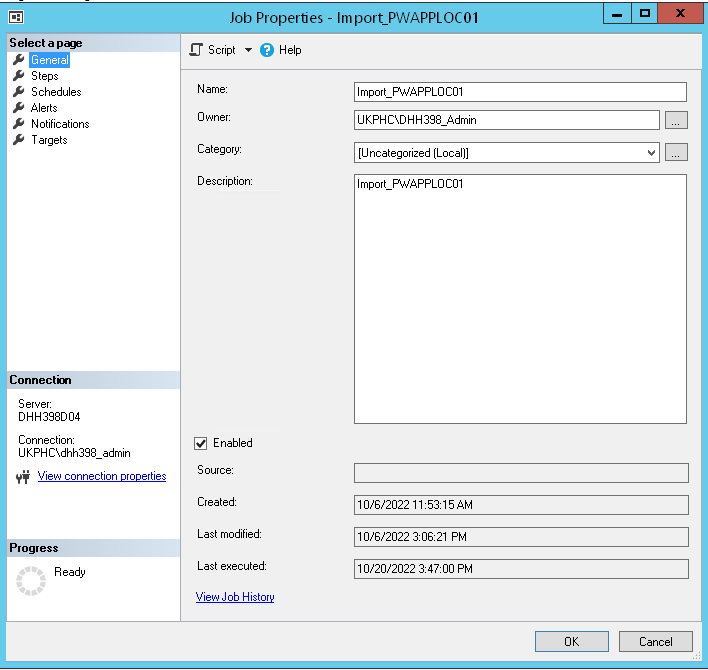
\includegraphics[width=0.7\textwidth, height=0.7\textheight,keepaspectratio]{immagini/M-schedulazione.png}
    \caption{Magazzino - Schedulazione aggiornamento database}
    \label{fig:M-Schedulazione}
\end{figure}
Per l’aggiornamento dei dati si è scritto il seguente codice:\\
    \texttt{delete from [dbo].[nome]\\
    DECLARE @SQLStr1 varchar(max)\\
    set @SQLStr1 =\\
    INSERT INTO [dbo].[nome] select *\\
    from OpenRowset('MSDASQL', select * FROM '\textit{nome}' )AS a\\
    EXECUTE(@SQLStr1);\\
    END}\\
\textit{Cioè prima si ripulisce il file e poi si importa nuovamente il tutto. L’eliminazione e la nuova importazione totale è più conveniente dell’aggiornamento dei singoli record in quanto si riduce il rischio di errore, si alleggerisce l’operazione non dovendo fare un continuo controllo tra i due file i quali potrebbero anche non essere ugualmente ordinati e ciò comporterebbe un ulteriore rallentamento.}\\
L’applicazione come da richiesta è stata sviluppata in un’unica schermata: oltre alla scannerizzazione e scrittura del barcode, nella parte alta si trovano le informazioni da visualizzare mentre nella seconda parte l’elenco delle locazioni specifiche di quell’articolo.\\
Nel database più record contengono lo stesso codice articolo e varia solo la locazione e relativa giacenza; quindi, sia per evitare di essere ripetitivi sia per fornire informazioni compatte a vista d’occhio in un’unica schermata, nella prima parte le informazioni vengono visualizzate una sola volta mediante questa formula nel suo contenitore generale:\\
\texttt{FirstN(Filter(Search([@PWAPPLOC01];TextInput1.Text;"IBLITM");\\
        Len(TextInput1.Text)=Len(TrimEnds(IBLITM)));1)
       }\\
\textit{Cerca nel database i record con il campo codice articolo (IBLITM) corrispondente a ciò che è scritto nella cella di input; filtra solo quelli che hanno lunghezza esattamente uguale alla lunghezza del codice inserito nella cella di input (calcolata con la funzione Trim per togliere gli spazi vuoti finali); filtra solo il primo record.}\\
Nella seconda parte per visualizzare l’elenco delle locazioni la formula è uguale ma senza il restringimento al primo record e quindi si filtra un elenco di record. Per la visualizzazione effettiva dei dati sono necessarie singole celle di testo impostate sulla specifica colonna; la \figurename \space \ref*{fig:M-Applicazione} mostra la schermata dell'applicazione
\begin{figure}[H]
    \centering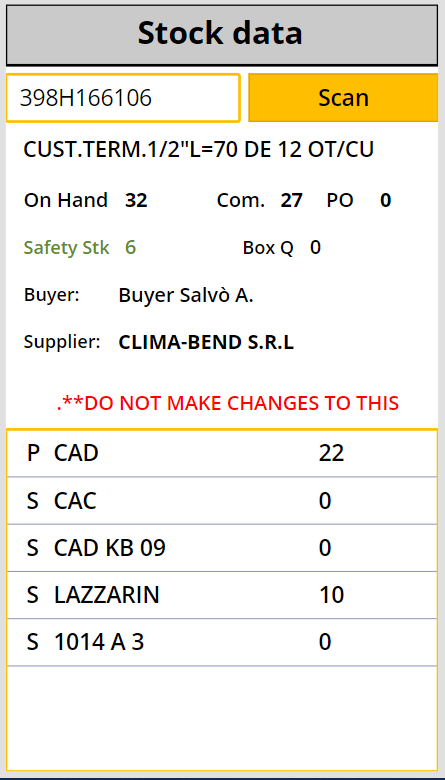
\includegraphics[width=0.4\textwidth, height=0.4\textheight,keepaspectratio]{immagini/M-applicazione.png}
    \caption{Magazzino - Unica schermata applicazione dati del magazzino}
    \label{fig:M-Applicazione}
\end{figure}

\backmatter
%\chapter{Glossario}
\begin{description}
    \item[Dashboard] in italiano si traduce cruscotto; raccoglie un insieme di dati, grafici, liste o tabelle che a colpo d'occhio forniscono un monitor sull'andamento di ciò che si sta analizzando.
    \item[DAX] Data Analysis Expressions è un linguaggio costituito da funzioni, operatori e costanti che si usano nelle formule o espressioni nei servizi di analisi dati per eseguire query e calcoli nei modelli di dati tabulari.
    \item[DB2] è un Relational Database Management System della IBM, si rimanda alla descrizione nella relativa sezione \ref*{tec:DB2}.
    \item[ERP] Enterprise Resource Planning è un sistema che si occupa della gestione e pianificazione aziendale delle risorse; si rimanda alla descrizione nella relativa sezione \ref*{tec:ERP}.
    \item[IBM] è l'azienda informatica più anziana, attiva già dalla fine dell'Ottocento, ed è tra le più grandi al mondo nel settore informatico.
    \item[IBM AS400] computer sviluppati dall'azienda IBM, commercializzati nel 1988, è un calcolatore che può servire migliaia di utenti contemporaneamente nell'esecuzione di programmi di gestione aziendale. Utilizza il sistema operativo OS400
    \item[Intranet]  è una rete privata aziendale che agevola la comunicazione interna consentendo di collaborare e semplificare i processi organizzativi.
    \item[Join] operazione tipica nei database, cioè unire due tabelle diverse. Esistono più tipologie di join e può essere imposta una condizione come filtro.
    \item[Linked Server] collegamento che permette di accedere ai dati gestiti da SQL Server o da altre sorgenti dati.
    \item[Microsoft Lists] è un software di Microsoft che permette di creare una lista di record, si rimanda alla descrizione nella relativa sezione \ref*{tec:Microsoft Lists}.
    \item[Microsoft SQL] è un Relational Database Management System di Microsoft, si rimanda alla descrizione nella relativa sezione \ref*{tec:Microsoft SQL}
    \item[ODBC] Open Database Connectivity è uno standard di Microsoft per permettere l'accesso e lo scambio dei dati.
    \item[OS400] sistema operativo sviluppato appositamente per i computer IBM AS400. Sistema operativo ad oggetti con già integrato un database DB2.
    \item[PowerPlatform] è la piattaforma sviluppata da Microsoft, basata sul principio low-code, affinchè gli utenti possano creare rapidamente e senza esserne esperti applicazioni, siti, report, automatizzare i processi; si rimanda alla descrizione nella relativa sezione \ref*{tec:PowerPlatform}
    \item[Power Apps] è un software di Microsoft, appartenente a PowerPlatform, che permette di realizzare applicazioni per tutti i dispositivi; si rimanda alla descrizione nella relativa sezione \ref*{tec:Power Apps}
    \item[Power Automate] è un servizio di Microsoft, appartenente a PowerPlatform, che permette di creare l'automazione dei processi organizzativi; si rimanda alla descrizione nella relativa sezione \ref*{tec:Power Automate}
    \item[Power Bi] è un software di Microsoft, appartenente a PowerPlatform, che realizza grafici per favorirne l'analisi; si rimanda alla descrizione nella relativa sezione \ref*{tec:Power BI} 
    \item[Query] interrogazione che viene svolta sul database al fine di estrapolare informazioni.
    \item[Record] è un oggetto composto da più campi di tipo eterogeneo tra loro, in ambito database e liste racchiude i campi di un elemento.
    \item[SharePoint] è una piattaforma di collaborazione, di Microsoft, permette di creare intranet; si rimanda alla descrizione nella relativa sezione \ref*{tec:SharePoint}.
\end{description}


%%\printglossary[type=main, title=Glossario, toctitle=Glossario]  NON FUNZIONA !!!
\end{document}